% DOC SETTINGS ===================================
\documentclass{article}
\usepackage[utf8]{inputenc}
\usepackage{steinmetz}
\usepackage{mathtools}  
\usepackage{multicol}
\usepackage{circuitikz}
\usepackage{listings}
\usepackage{geometry}
\usepackage{fancyhdr}
\pagestyle{fancy}
\lhead{ECE2564 Homework 3}
\rhead{Kavin Thirukonda 2021}
\fancyheadoffset{0mm}
 \geometry{
 a4paper,
 total={170mm,257mm},
 left=20mm,
 top=25mm,
 }
\mathtoolsset{showonlyrefs} 
\cfoot{}
% DOC SETTINGS ===================================
\begin{document}
\begin{center}
    “I have neither given nor received unauthorized assistance on this assignment.”
    
    
\includegraphics[width = .1\textwidth]{Signature.jpg}
\end{center}
\section*{Problem 0}
\begin{center}
    Github ID: kavnthir\\
    Github ID Number: 63033113
\end{center} 
\section*{Problem 1}
\subsection*{(a)}
\begin{center}
        \lstset{language=C}
        \lstset{frame=lines}
        \lstset{label={lst:code_direct}}
        \lstset{basicstyle=\footnotesize}
        \begin{lstlisting}
#include <stdio.h>

//This is so that we can use BIT0, BIT1,etc. macros as well as types bool, keywords true, false
#include <ti/devices/msp432p4xx/driverlib/driverlib.h>

void main() {

    unsigned int starting_value = 0XFEDCBA95;
    bool test_v;

    unsigned k = starting_value;

    unsigned int l = k & BIT0;


    //TODO #1:

    k = k | BIT2 | BIT3;

    //TODO #2: 

    k = ((k | BIT6 | BIT5) & ~BIT7) & ~BIT4;

   //TODO #3: 

    k = ((k ^ BIT5) | BIT1) & ~BIT0;

    //TODO #4: 
   
    test_v = ((BIT(31) & k) == BIT(31)) && ((BIT0 & k) == 0);

    if (test_v)
        printf("The test variable is true.\n");
    else
        printf("The test variable is false.\n");

}
        \end{lstlisting}
\end{center}
\newpage
\subsection*{(b)}
\begin{center}
    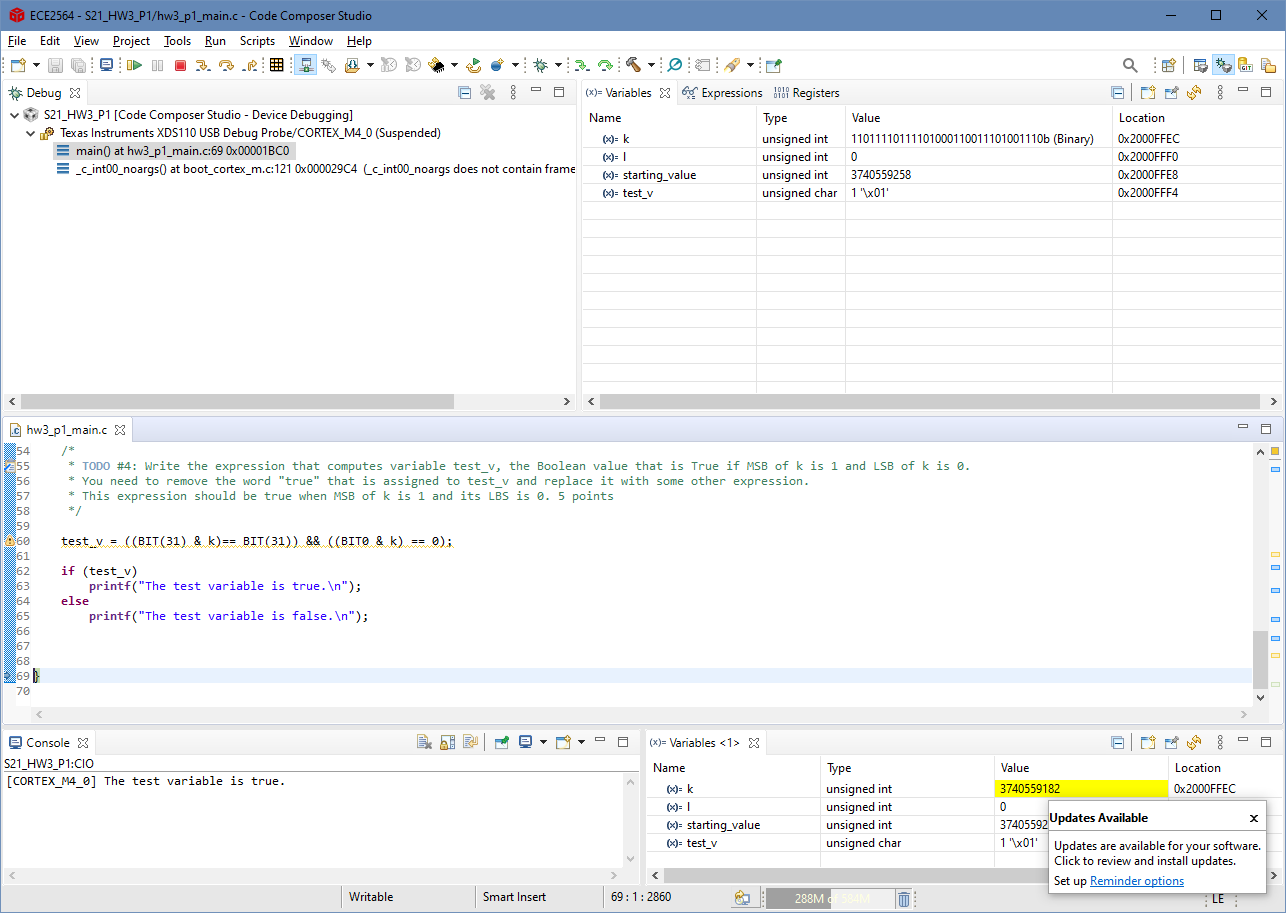
\includegraphics[width = \textwidth]{part1.png}
\end{center}
\newpage
\section*{Problem 2}
\subsection*{(a)}
Show the value of an LSR that programs a light with red color and high intensity without flicker. Show the value both in binary and hex. 
\begin{center}
    Binary: 0b11000000
    Hex: 0xC0
\end{center}
\subsection*{(b)}
Translate what it means if the value of an LSR is 0xBE.
\begin{center}
    Hex: 0xBE \\
    Binary: 0b10111110 \\
    Intensity: medium \\
    Color: yellow \\
    Flicker: true
\end{center}
\subsection*{(c)}
\begin{center}
        \lstset{language=C}
        \lstset{frame=lines}
        \lstset{label={lst:code_direct}}
        \lstset{basicstyle=\footnotesize}
        \begin{lstlisting}
// TODO #1: 
#define COLOR_MASK (BIT4 | BIT5)
#define INTENSITY_MASK (BIT6 | BIT7)
#define FLICKER_MASK BIT3
// TODO #2:
#define COLOR_BIT_POS 4
#define INTENSITY_BIT_POS 6
#define FLICKER_BIT_POS 3
// TODO #3: 
typedef enum {RED, GREEN, BLUE, YELLOW} color_t;
typedef enum {INT_OFF, INT_LOW, INT_MED, INT_HIGH} intensity_t;
typedef enum {FLICK_OFF, FLICK_ON} flickering_t;
// TODO #NAN: 
typedef unsigned char LSR_t;
// TODO #4:
typedef struct {
    LSR_t lightSetting;           // the setting of the light
    unsigned int x;               // the x coordinate of the light
    unsigned int y;               // the y coordinate of the light
} light_t;
        \end{lstlisting}
\end{center}
\newpage
\subsection*{(d)}
\begin{center}
        \lstset{language=C}
        \lstset{frame=lines}
        \lstset{label={lst:code_direct}}
        \lstset{basicstyle=\footnotesize}
        \begin{lstlisting}
// TODO #5:
color_t getColorSetting(LSR_t inLSR) {
    color_t colorSetting = (color_t) ((inLSR & COLOR_MASK) >> COLOR_BIT_POS);
    return colorSetting;
}
intensity_t getIntensitySetting(LSR_t inLSR) {
    intensity_t intensitySetting = (intensity_t)((inLSR & INTENSITY_MASK) >> INTENSITY_BIT_POS);
    return intensitySetting;
}
flickering_t getFlickeringSetting(LSR_t inLSR) {
    flickering_t FlickeringSetting = (flickering_t)((inLSR & FLICKER_MASK) >> FLICKER_BIT_POS);
    return FlickeringSetting;
}
        \end{lstlisting}
\end{center}
\subsection*{(e)}
\begin{center}
    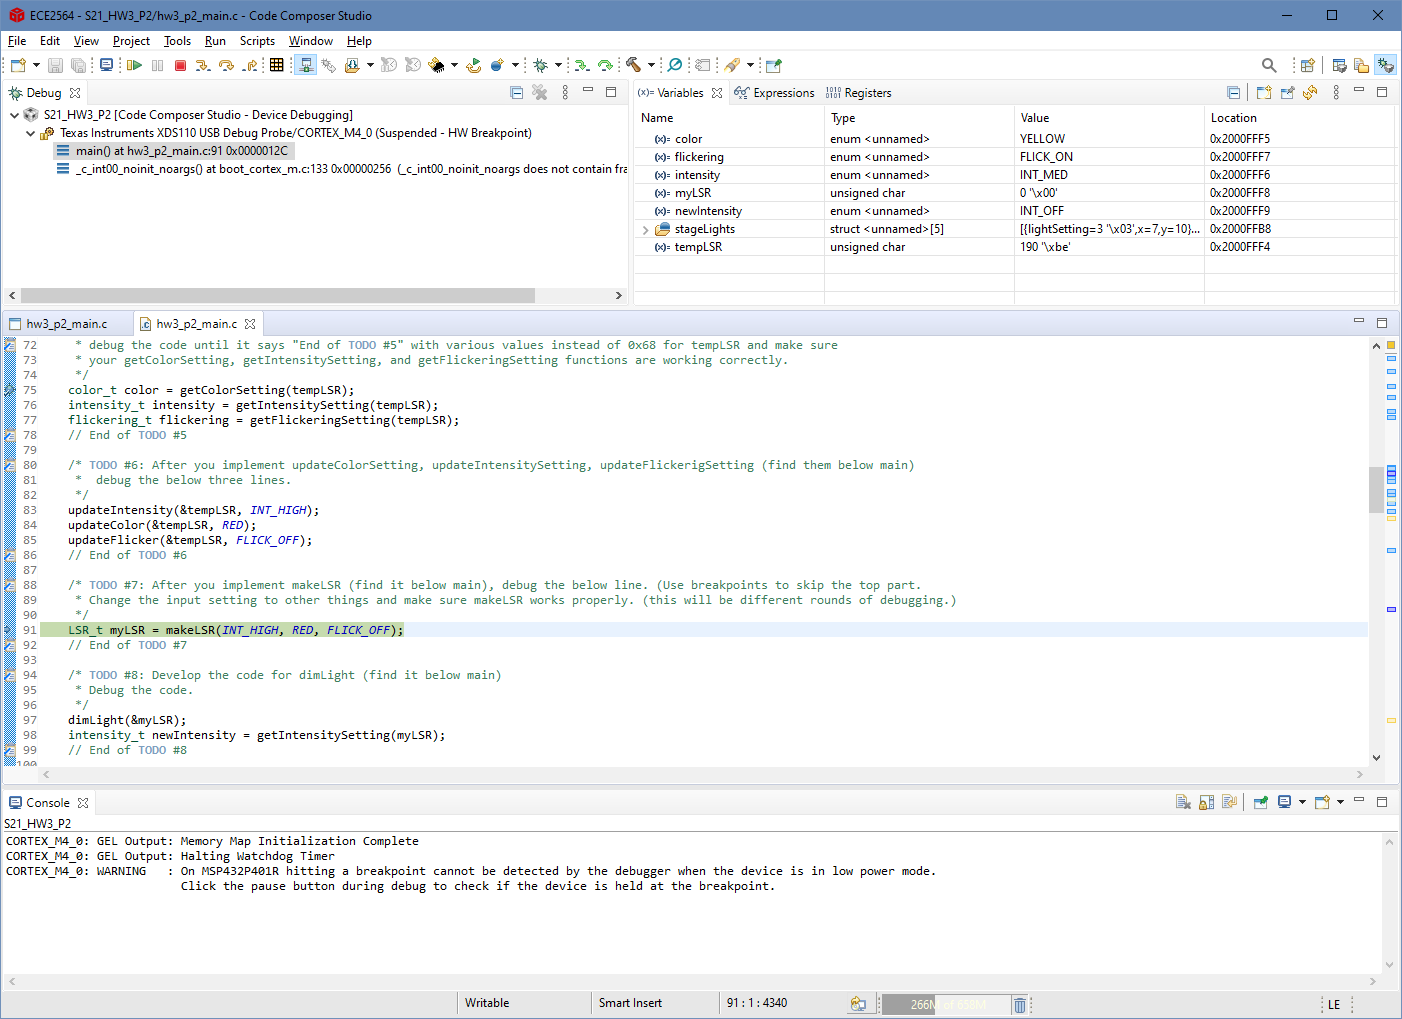
\includegraphics[width = \textwidth]{e.png}
\end{center}
\newpage
\subsection*{(f)}
\begin{center}
         \lstset{language=C}
        \lstset{frame=lines}
        \lstset{label={lst:code_direct}}
        \lstset{basicstyle=\footnotesize}
        \begin{lstlisting}
// TODO #6:
void updateIntensity(LSR_t* LSR_p, intensity_t newIntensity) {
    *LSR_p = (*LSR_p & ~INTENSITY_MASK)|((newIntensity) << INTENSITY_BIT_POS);
}
void updateColor(LSR_t* LSR_p, color_t newColor) {
    *LSR_p = (*LSR_p & ~COLOR_MASK)|((newColor) << COLOR_BIT_POS);
}
void updateFlicker(LSR_t* LSR_p, flickering_t newFlicker) {
    *LSR_p = (*LSR_p & ~FLICKER_MASK)|((newFlicker) << FLICKER_BIT_POS);
}
        \end{lstlisting}
\end{center}
\subsection*{(g)}
\begin{center}
    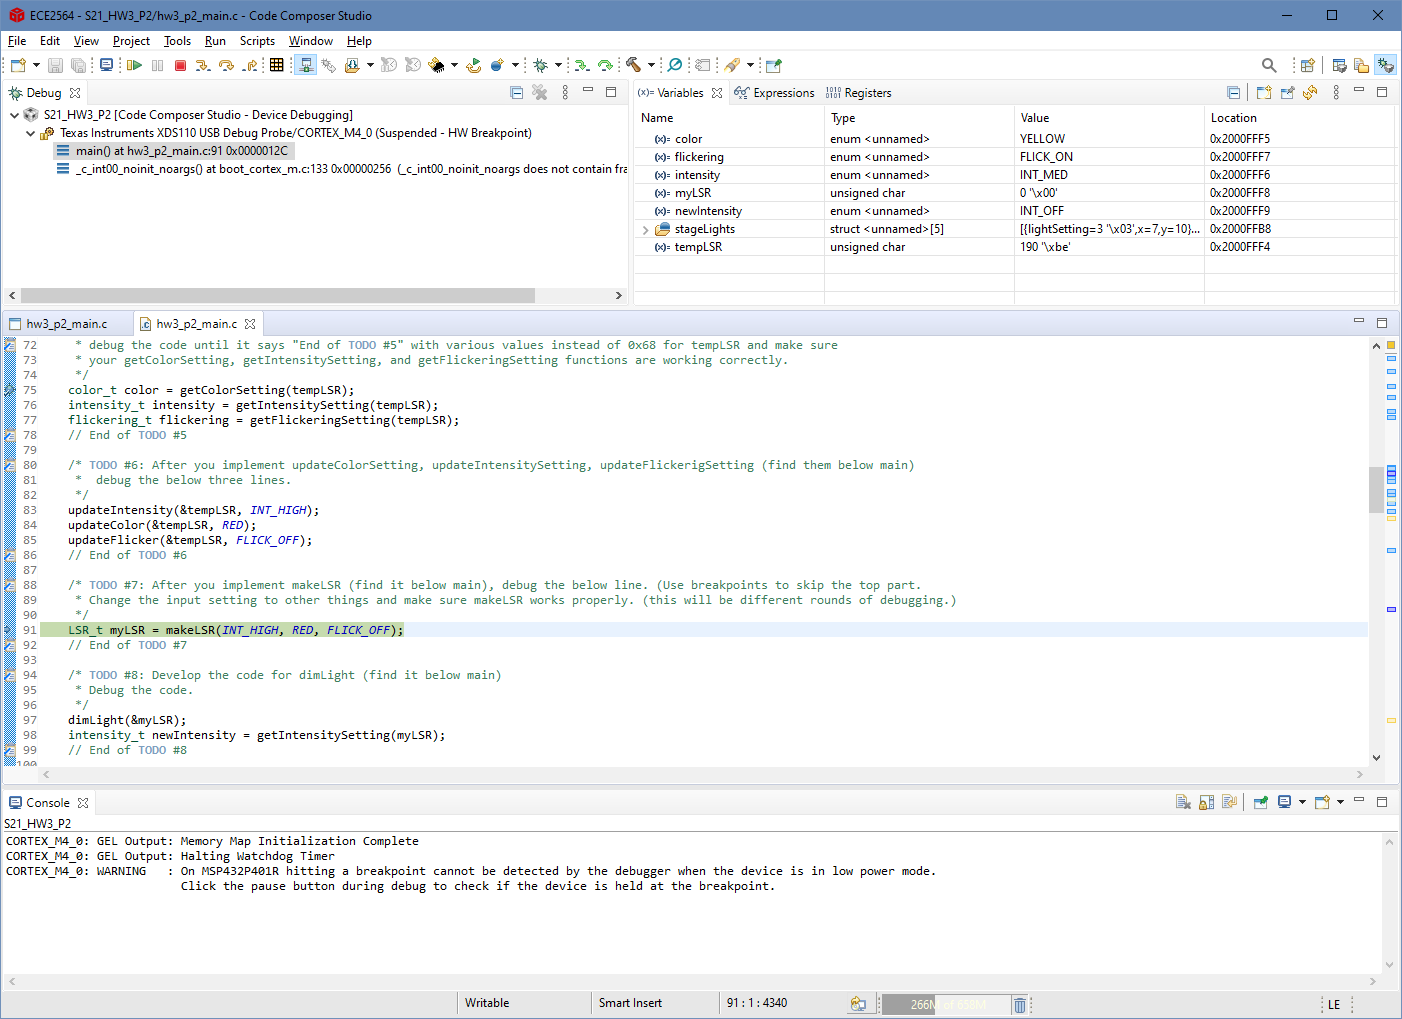
\includegraphics[width = \textwidth]{e.png}
\end{center}
\newpage
\subsection*{(h)}
\begin{center}
         \lstset{language=C}
        \lstset{frame=lines}
        \lstset{label={lst:code_direct}}
        \lstset{basicstyle=\footnotesize}
        \begin{lstlisting}
// TODO #7:
LSR_t makeLSR(intensity_t newIntensity, color_t newColor, flickering_t newFlickering) {
    LSR_t newLSR = 0;
    updateIntensity(&newLSR, newIntensity);
    updateColor(&newLSR, newColor);
    updateFlicker(&newLSR, newFlickering);
    return newLSR;
}
        \end{lstlisting}
\end{center}
\subsection*{(i)}
\begin{center}
    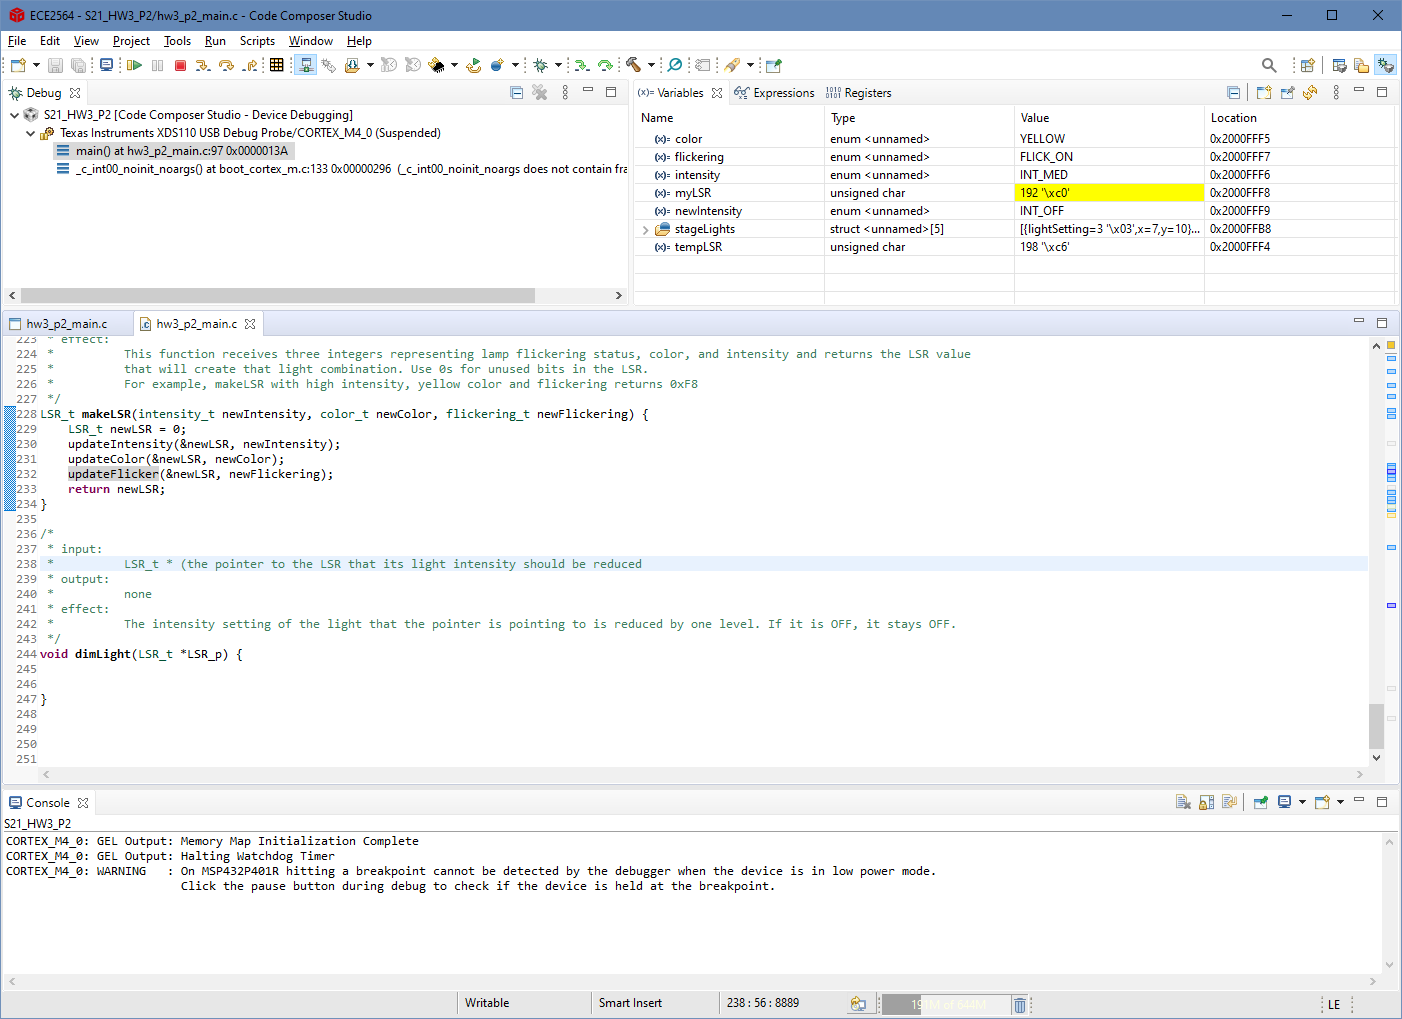
\includegraphics[width = \textwidth]{i.png}
\end{center}
\newpage
\subsection*{(j)}
\begin{center}
        \lstset{language=C}
        \lstset{frame=lines}
        \lstset{label={lst:code_direct}}
        \lstset{basicstyle=\footnotesize}
        \begin{lstlisting}
void dimLight(LSR_t *LSR_p) {
    intensity_t tempIntensity = getIntensitySetting(*LSR_p);
    switch (tempIntensity){
    case INT_OFF:
        break;
    case INT_LOW:
        updateIntensity(LSR_p, INT_OFF);
        break;
    case INT_MED:
        updateIntensity(LSR_p, INT_LOW);
        break;
    case INT_HIGH:
        updateIntensity(LSR_p, INT_MED);
        break;
    }
}
        \end{lstlisting}
\end{center}
\subsection*{(k)}
\begin{center}
    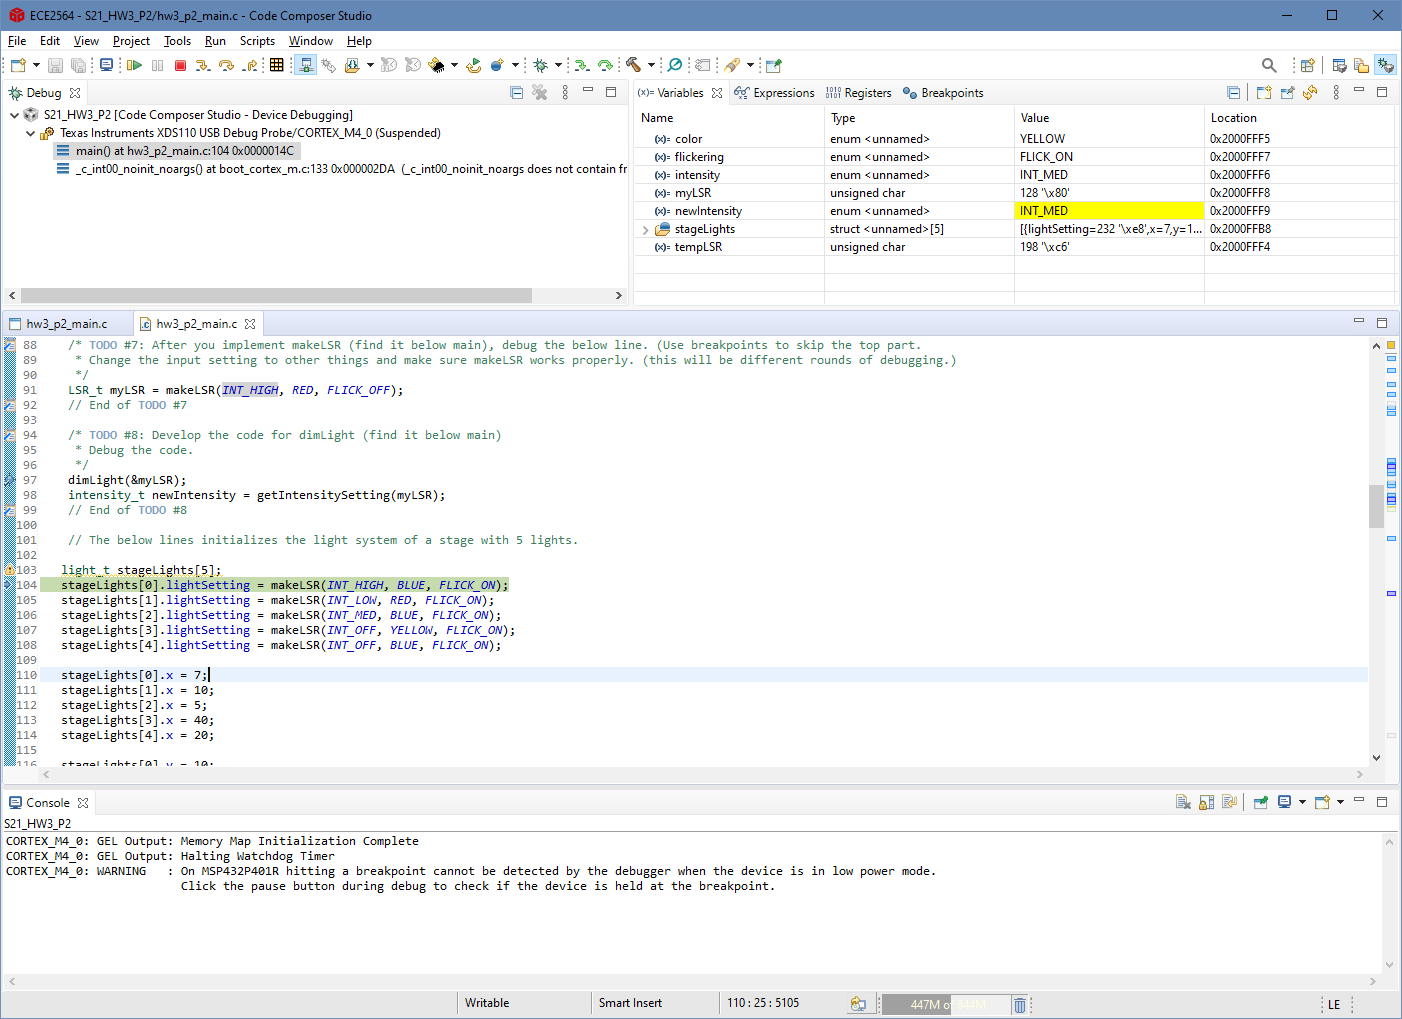
\includegraphics[width = \textwidth]{k.png}
\end{center}
\newpage
\subsection*{(l)}
\begin{center}
        \lstset{language=C}
        \lstset{frame=lines}
        \lstset{label={lst:code_direct}}
        \lstset{basicstyle=\footnotesize}
        \begin{lstlisting}
int i = 0;
for(i = 0; i < 5; i++){
   if(stageLights[i].x < 20){
       dimLight(&stageLights[i]);
   }
   if((stageLights[i].x < 30) && (stageLights[i].y <30)){
       updateColor(&stageLights[i], RED);
   }else{
       updateColor(&stageLights[i], YELLOW);
   }
}
        \end{lstlisting}
\end{center}
\subsection*{(m)}
\begin{center}
    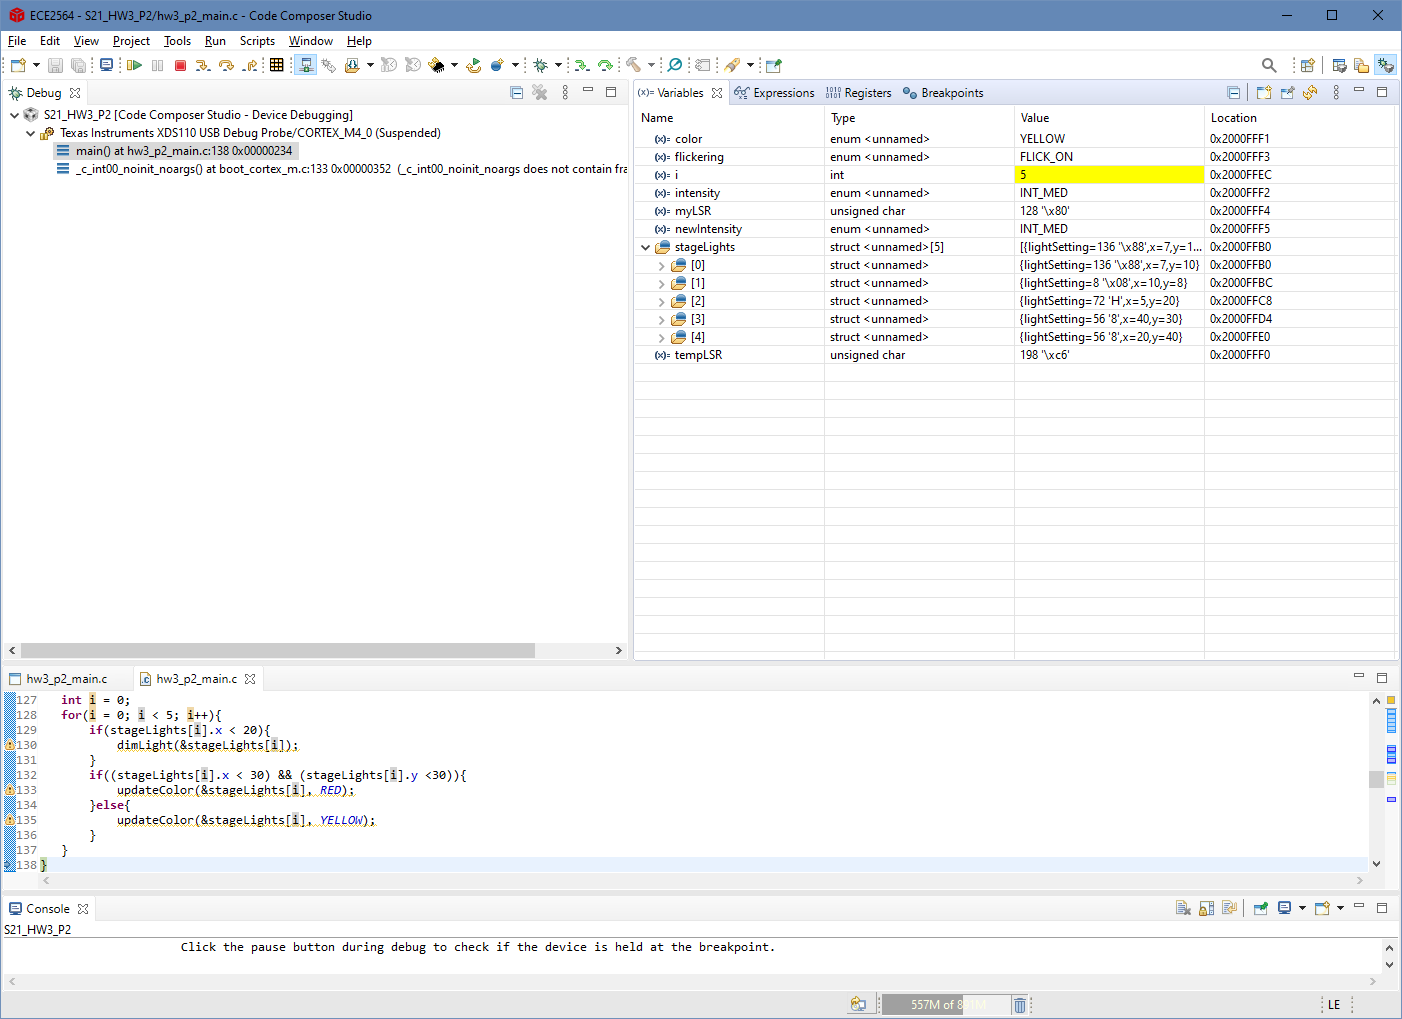
\includegraphics[width = \textwidth]{m.png}
\end{center}
\end{document}
